\chapter{Présentation de l'entreprise}
\chaptermark{Présentation Générale}
\minitoc
\newpage
 
\section{L’histoire de Transaction Connect}
Transaction Connect est une start-up française fondée en 2016 par Didier GASTÉ après ses huit années passées chez le leader de l’immobilier commercial européen Unibail-Rodamco dans le secteur du digital. Il s’associe à son cofondateur Maxime Dellerie pour inventer une technologie permettant de transformer tout moyen de paiement électronique en une carte de fidélité. Avec un capital de 30.315€, Transaction Connect commence ses activités le 08 septembre 2016 de manière officielle et fixe son siège social au 86 rue du Faubourg Saint Denis 75010 Paris. En moins d’une année son capital passe à 31.575€. 

Dans ses activités la start-up estime une perte de moitié des capitaux propres et est sous la menace de dissolution. Au terme de l’Assemblée Générale ordinaire du 28 juin 2019, il a été décidé de ne pas dissoudre la société bien que ses capitaux propres soient devenus inférieurs à la moitié du capital social. Aux termes du PV des Décisions du 25 juillet 2019, Le Président a constaté la réalisation d’une augmentation du capital social d’un montant de 9.287€, ce qui permet au capital de revenir à 40.862€ et qui prend effet au 25 juillet 2019. En décembre 2020, par la décision du président , Transaction Connect a vu son siège social transféré au 210 Quai de Jemmapes, Bureaux 2e étage 75010 et prend effet le 31 décembre 2020.

En quelques mois d’activités dans cette nouvelle adresse, suite à la décision du président fondateur, la start-up retourne à son ancienne adresse 86 rue du Faubourg Saint Denis 75010 Paris

\newpage
\section{Chiffres de Transaction Connect}
\begin{figure}[h]
\begin{center}
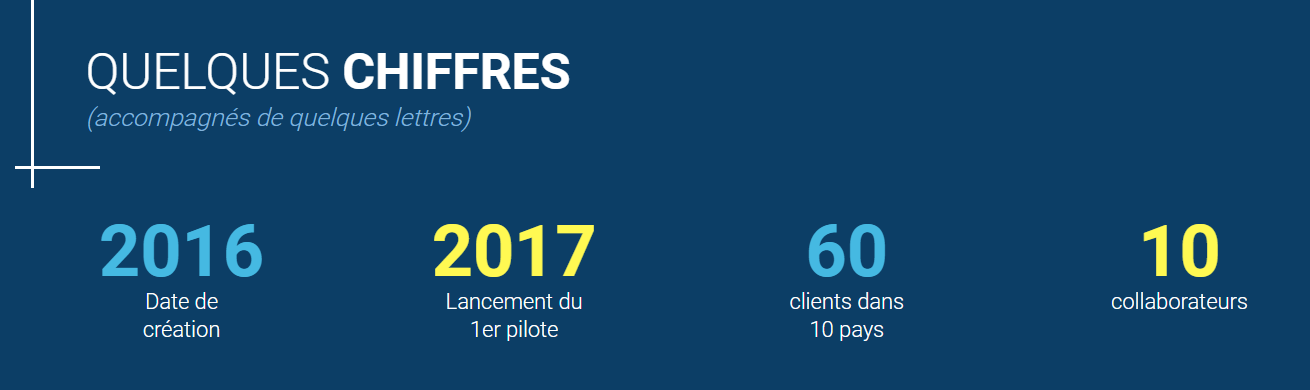
\includegraphics[width=15cm,height=6cm]{images/chiffres_tc.png}
\caption[Chiffres sur actuels sur l'évolution de Transaction Connect]{Chiffres sur actuels sur l'évolution de Transaction Connect}
\label{monlabel}
\end{center}
\end{figure}

\begin{figure}[h]
\begin{center}
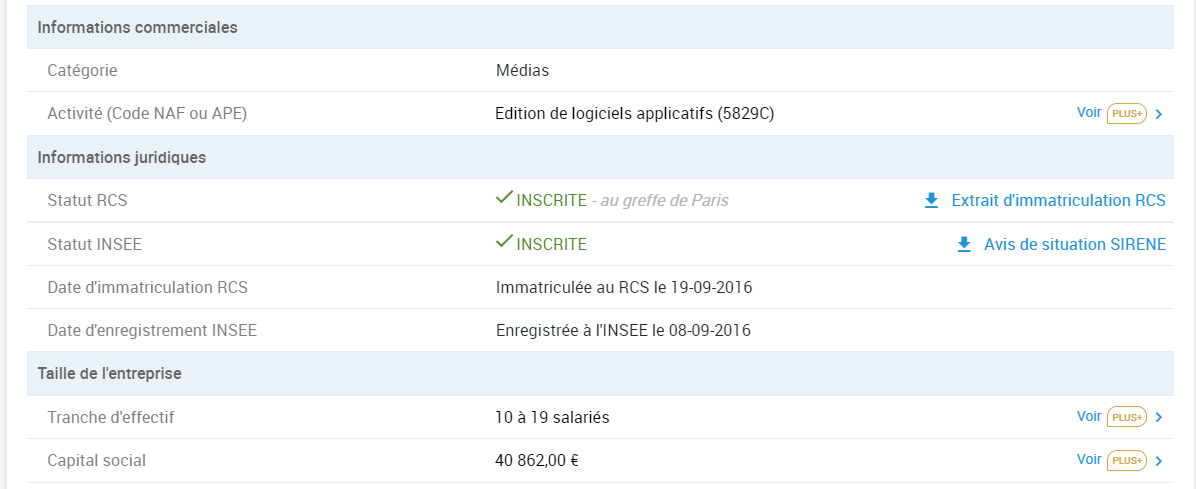
\includegraphics[width=15cm,height=9cm]{images/chiffre_affaire.png}
\caption[Informations sur la start-up Transaction Connect]{Informations sur la start-up Transaction Connect}
\label{monlabel}
\end{center}
\end{figure}
\newpage

\section{Les Clients de Transaction Connect}
\begin{enumerate}
\item Clients foncières B2B;
En 2017, Transaction Connect a signé son premier contrat avec le géant européen de l’immobilier commercial Unibail Rodamco en testant sa solution de la mise en relation d’un moyen de paiement à un programme de fidélité qui permet l’accès à des données de comportement d’achat. Par la suite, la start-up ne cesse de signer d’autres contrats et compte aujourd’hui une vingtaine de clients foncières en Europe notamment SOCRI, Nepi, Rockcastle, Hyper U, Eurocommercial, Accessite, CHEESE, …

Ces foncières bénéficient donc de deux modes d’intégration sur contrat:
\begin{itemize}
\item Intégration en White Label\\
Les clients Business inscrits en White Label bénéficient des services comme la page web de connexion, la synchronisation des comptes bancaires de leurs clients, l’enrichissement des données récupérées, la fourniture des dashboard analytics, la notification et envoie des récompenses.
\item Intégration en External Front\\
Pour les clients foncières qui optent à ce mode d’intégration Transaction connect fournit tous les services précédents sauf la page web de connexion et la notification de cashback. Dans le premier cas le foncier fait appelle à Transaction Connect à lui mettre en place la solution avec tous les services alors dans ce cas le client dispose de certains services en interne.

\begin{figure}[h]
\begin{center}
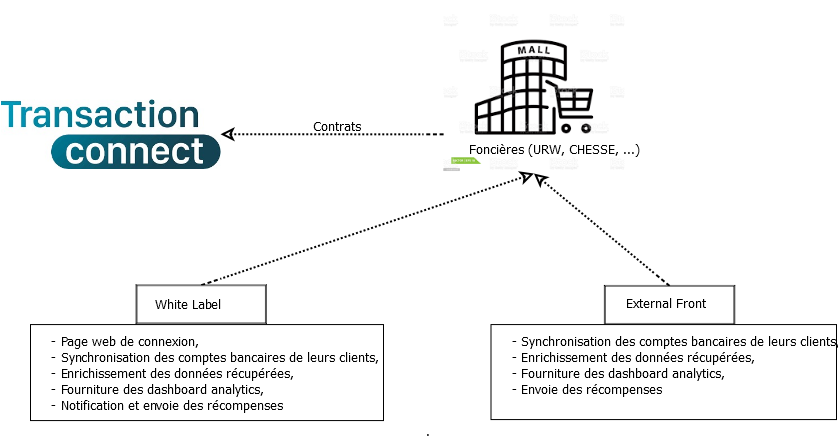
\includegraphics[width=15cm,height=9cm]{images/business_links.png}
\caption[Modes d'intégration des foncières]{Modes d'intégration des foncières}
\label{monlabel}
\end{center}
\end{figure}
\end{itemize}
\newpage

\item Clients acheteur B2C\\
Les clients acheteurs sont la source génératrice de la matière première de transaction Connect. Ils s’inscrivent à un programme de fidélité qu' offre un Centre Commercial en donnant leur consentement sur le mode de connexion de leur transaction. Après avoir enrichi ces transactions en appliquant les solutions mise en place par Transaction Connect, les clients foncières s’en servent pour prendre des décisions et des recommandations. Les  clients bénéficient au choix de trois modes de connexion des données d’achats. 
\begin{itemize}
\item Account Linking\\
Les clients sous cette formule de connexion acceptent que Transaction Connect accède à l’historique de toutes ses transactions à travers leur Banque. En effet, Transaction ne reçois pas des informations personnelles du client, elle a accès à certaines informations intéressante notamment: un label de description du produit acheté
Le nom du retail chez qui il a effectué l’achat, la date de transaction, le montant, …
Exemple: “CB CARREFOUR 045 02/03/2021 10€”

\item Card Linking \\
Dans cette formule de connexion, le client désire transmettre seulement les transactions effectuées dans les Centres dans lesquels ils sont inscrits.
\item Receipt Linking \\
Pour les clients qui hésitent à donner accès à leur compte bancaire, ils ont la possibilité de scanner les tickets de caisse et de les envoyer. Transaction se charge d’extraire les informations pertinentes afin de le considérer comme une transaction.

\end{itemize}
\newpage
Le client en contrepartie reçoit des récompenses après chaque montant dépensé dans le Centre dans lequel il est fidélisé. En Pologne par exemple, le client cumule des points pour les achats  supérieurs à 30 PLN, reçoit 30 points pour chaque achat de ce type. Il se voit récompensé par virement sur son compte 30 PLN à chaque 300 points atteints.
\begin{figure}[h]
\begin{center}
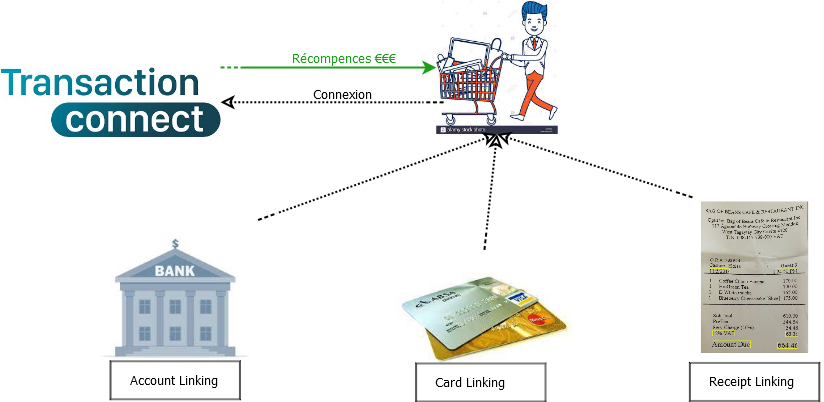
\includegraphics[width=15cm,height=9cm]{images/client_links.png}
\caption[Modes de connexion des Clients aux programmes de fidélités]{Modes de connexion des Clients aux programmes de fidélités}
\label{monlabel}
\end{center}
\end{figure}
\end{enumerate}
\newpage

\section{Les services clés}
 Transaction Connect propose une solution révolutionnaire aux centres commerciaux qui remplacent les cartes de fidélité en se basant sur les données d’achats des clients. 
En rattachant un moyen de paiement à une entité,  Transaction Connect permet aux acteurs du commerce physique, d’améliorer leur connaissance client et de proposer des expériences innovantes, fluides et personnalisées à leurs clients. Les services qu’offre Transaction Connect:
\begin{itemize}
\item Page web de connexion\\
Pour les clients foncières en white label, Transaction Connect leur fournit une page web que vont utiliser leurs clients acheteurs afin de s’inscrire aux fidélités et de charger des tickets de caisse.
\item Synchronisation des comptes bancaires de leurs clients:\\
Transaction Connect intervient aussi dans la récupération des données de transactions auprès des fournisseurs (Fidel, Fintecture, Manual, Salt Edge Dsp2, Swedbank, Budget Insight) qui sont en contact avec les Banques. 
\item Enrichissement des données récupérées:\\
Grâce aux différentes solutions de Transactions Connects les données sont enrichies afin de définir la source de la transaction notamment le Centre commercial hôte, le retailer qu’appartient le magasin d’achat et le magasin lui-même..
\item Fourniture des dashboard analytics:\\
Après que les données sont enrichies, on construit des indicateurs de performances et d’évolution afin de comprendre le comportement d’achat des clients.
\item Notification et envoie des récompenses:\\
Lorsque un client acheteur est éligible à percevoir une récompense, Transaction Connect envoie un message d’information du montant débloqué et envoie un virement du montant correspondant au client.
\end{itemize}
\newpage

\section{Transaction Connect en interne}
\begin{enumerate}
\item L’ équipe d’accueil:\\
Tout d’abord, Transaction connect compte deux équipes techniques notamment l’équipe de Plateforme et l’équipe de Data.
Tout mon parcours chez Transaction Connect s’est passé au sein de l’équipe data de composé de six membres. Au sein de l’équipe, on retrouve deux catégories de profils: les data scientistes et les data analystes. Les tâches analytiques sont subdivisées en deux: les tâches à destination des clients externes notamment les foncières qui s’en servent pour suivre la performance d’accueil des clients. La deuxième analyse gérée par un autre membre de l’équipe vise à monitorer les qualités d’affectation des transactions en interne. Les Data scientist interviennent dans la mise en place des algorithmes de machine learning permettant d’enrichir des transactions.

\item Organisation de travail: le scrum Agile\\
Scrum est une méthode agile pour la gestion de projet informatique et a pour objectif d’améliorer la productivité d’une équipe. C’est un cadre de travail au sein duquel les acteurs peuvent aborder des problèmes complexes et adaptatifs, en livrant de manière efficace et créative des produits tout en créant de la valeur ajoutée. Le sprint dure deux semaines et sur cette période chacun travail sur une ou plusieurs tâches dans le but de fournir un résultat en fin de sprint.

\item Outils techniques:\\
Dans le but de réaliser mes missions au sein de Transaction Connect, cette dernière a mis à ma disposition un ordinateur portable. Comme outils technique ou de communication on dispose entre autres de DataGrip, Pycharm, Slack, Dashlane, VPN,...
\end{enumerate}







